\documentclass[letterpaper]{article}

\usepackage{amsmath}
\usepackage{gensymb}
\usepackage[vmargin=1in,hmargin=1.25in]{geometry}
\usepackage{graphicx}
\usepackage{hyperref}
\usepackage{microtype}
\usepackage{lmodern}
\usepackage{tikz}
\usetikzlibrary{matrix}

\author{Philip Pham}
\title{\Large ECE/CSE 576, Spring 2019 Homework 2: Creating Panoramas}
\date{\today}

\begin{document}
\maketitle

\section{Harris Corner Detector}
\label{sec:harris}
Gaussian blurring was applied with $\sigma = 2$. The Harris response threshold
was $50$, and non-maximal suppression was done with a $5 \times 5$
window. Detected corners are denoted with a red cross. As a sanity check, we
apply the algorithm to \texttt{Boxes.png}.

\begin{center}
  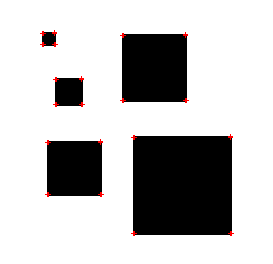
\includegraphics{1a.png}  
\end{center}

\begin{center}
  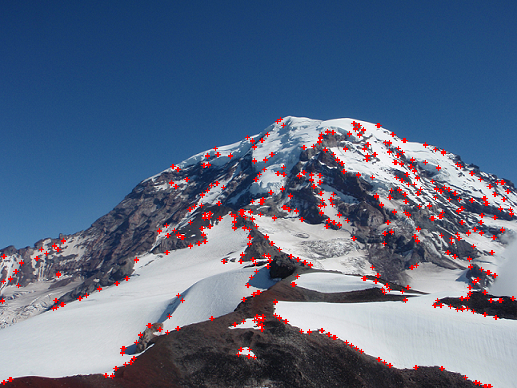
\includegraphics[width=0.73\textwidth]{1b.png}
  
  Applied to \texttt{Rainier1.png}.
\end{center}

\begin{center}
  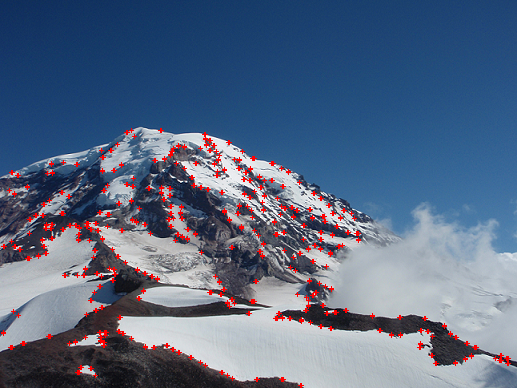
\includegraphics[width=0.73\textwidth]{1c.png}
  
  Applied to \texttt{Rainier2.png}.
\end{center}

\section{Match Corner Points}

The $l_1$ norm applied to the feature descriptor was used to find matching
corner points in the other image.

\begin{center}
  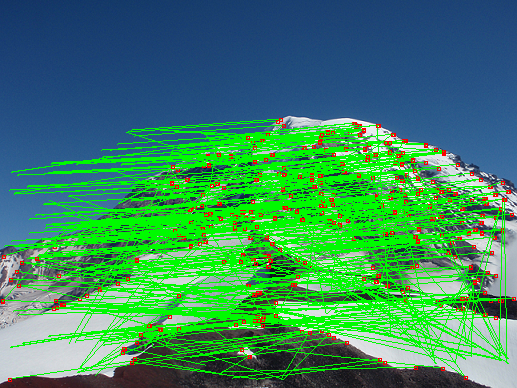
\includegraphics[width=0.85\textwidth]{2a.png}
  
  All matching corner points in \texttt{Rainier1.png}.
\end{center}

\begin{center}
  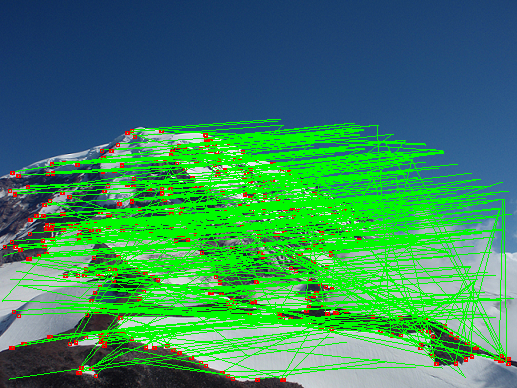
\includegraphics[width=0.85\textwidth]{2b.png}
  
  All matching corner points in \texttt{Rainier2.png}.
\end{center}

\section{RANSAC}

Homographies were sampled by choosing 4 matches. The homography with the largest
number of inliers was chosen.

\begin{center}
  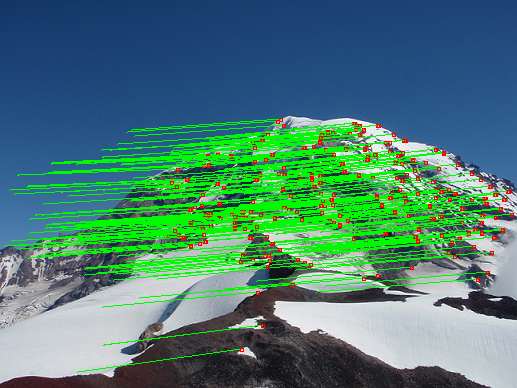
\includegraphics[width=0.85\textwidth]{3a.png}
  
  Matches from the homography with the largest number of inliers in
  \texttt{Rainier1.png}.
\end{center}

\begin{center}
  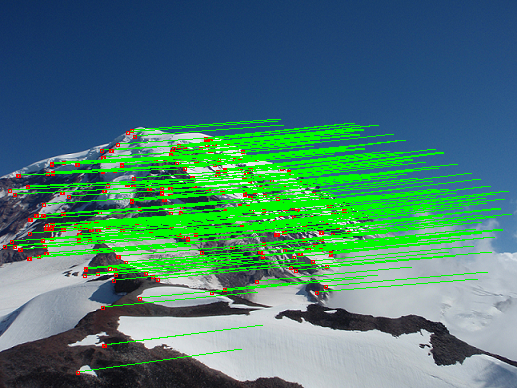
\includegraphics[width=0.85\textwidth]{3b.png}
  
  Matches from the homography with the largest number of inliers in
  \texttt{Rainier2.png}.
\end{center}

\section{Stitch}
\label{sec:stitch}

A flat panorama was made by using the first image as the reference coordinate
system.

\begin{center}
  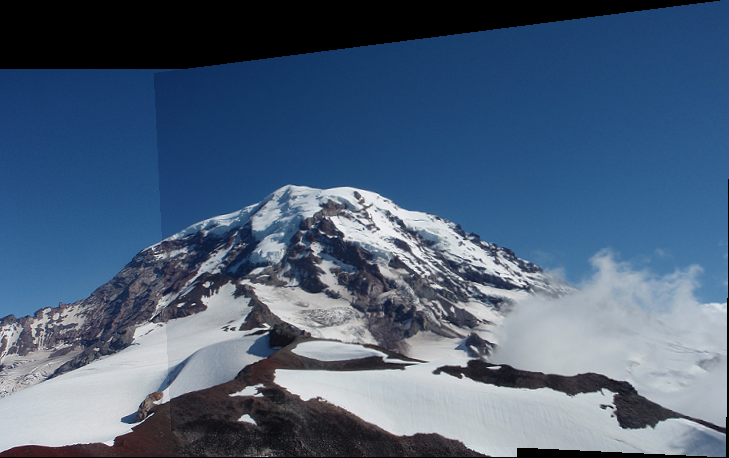
\includegraphics[width=\textwidth]{4.png}
  
  The result of stitching \texttt{Ranier1.png} and \texttt{Ranier2.png}.
\end{center}

\section*{Bell: Complete Mt. Ranier Panorama}

The same technique in Section \ref{sec:stitch} can be applied repeatedly to get a
complete panorama.

\begin{center}
  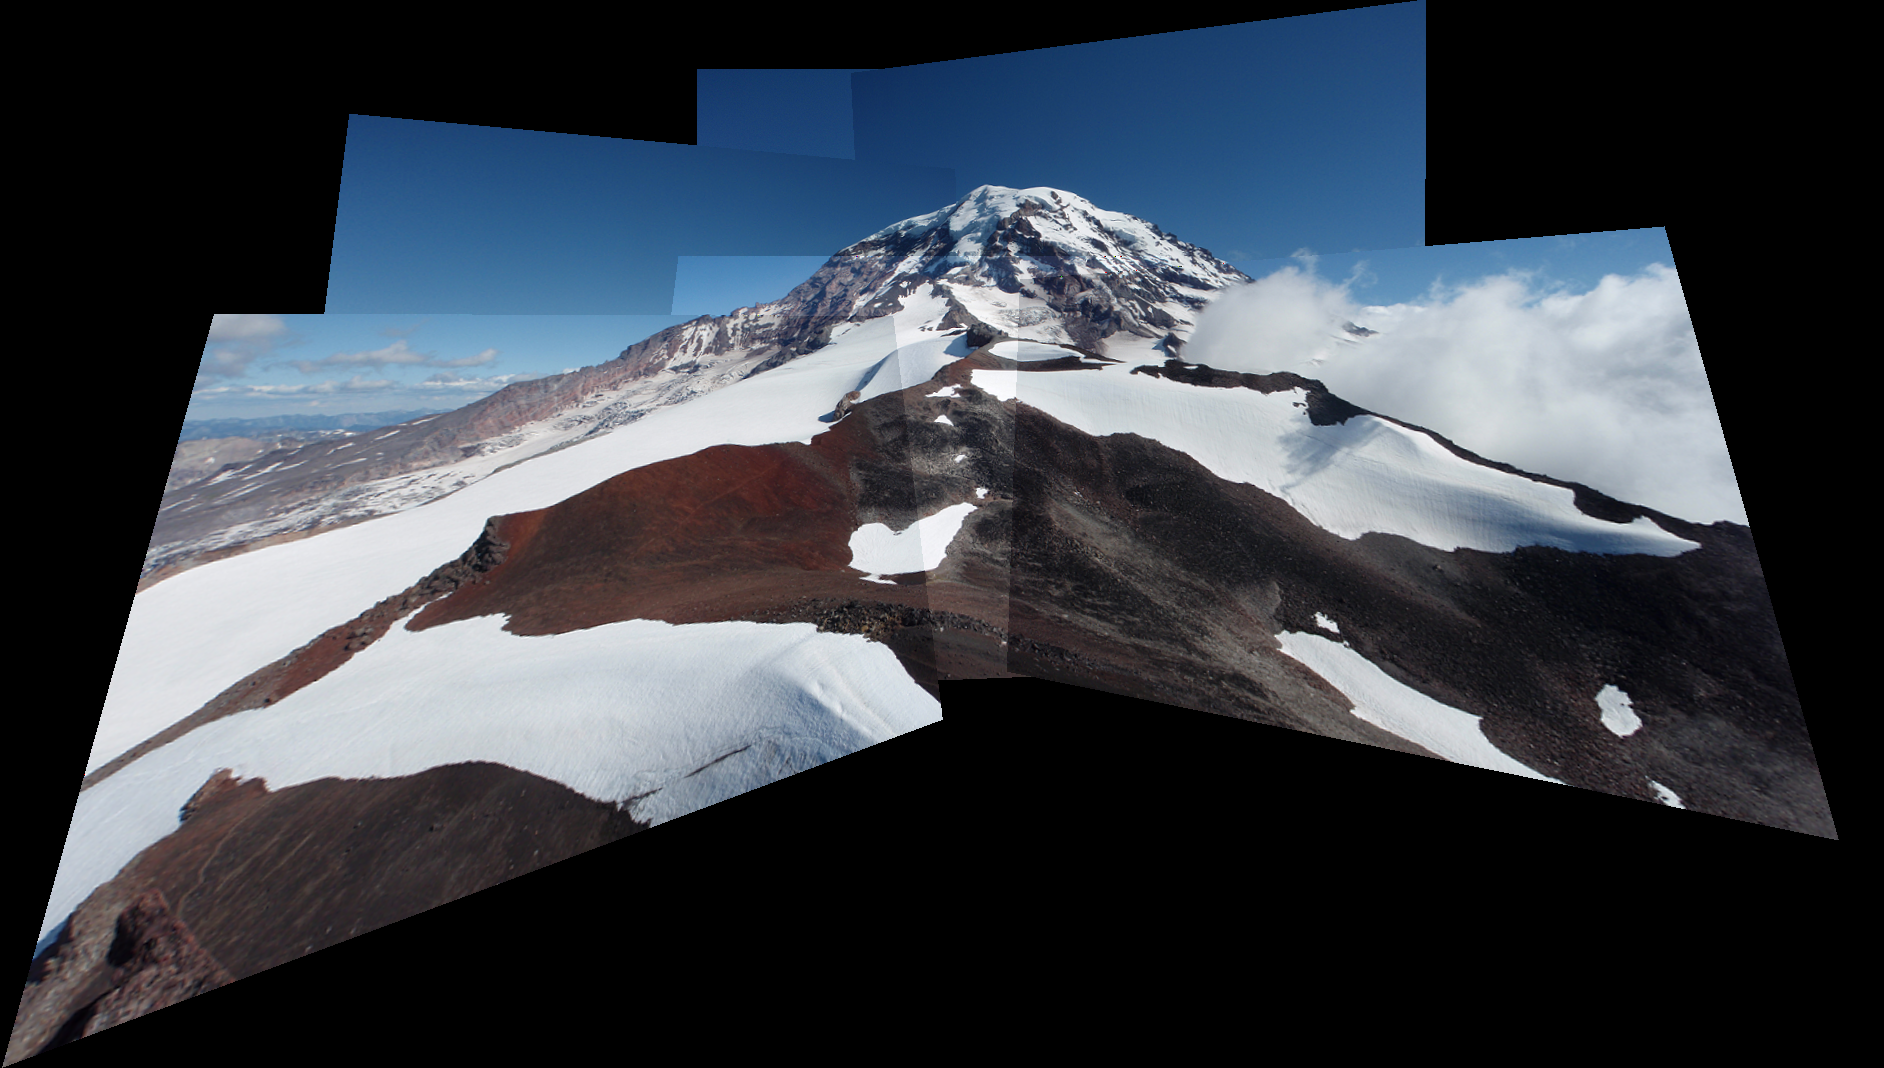
\includegraphics[width=\textwidth]{all_stitched.png}
  
  The result of stitching \texttt{Ranier1.png}, \texttt{Ranier2.png},
  \texttt{Ranier3.png}, \texttt{Ranier4.png}, \texttt{Ranier5.png}, and
  \texttt{Ranier6.png}.
\end{center}

\section*{Whistle: My Own Panorama}

I took pictures of my office building with my cell phone camera and stiched them
together. Images were resized to $480 \times 640$, but otherwise, untouched.

\begin{center}
  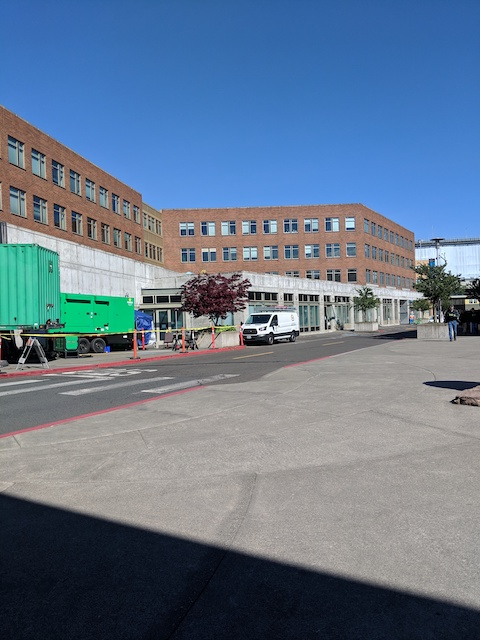
\includegraphics[width=0.32\textwidth]{google3.jpg}
  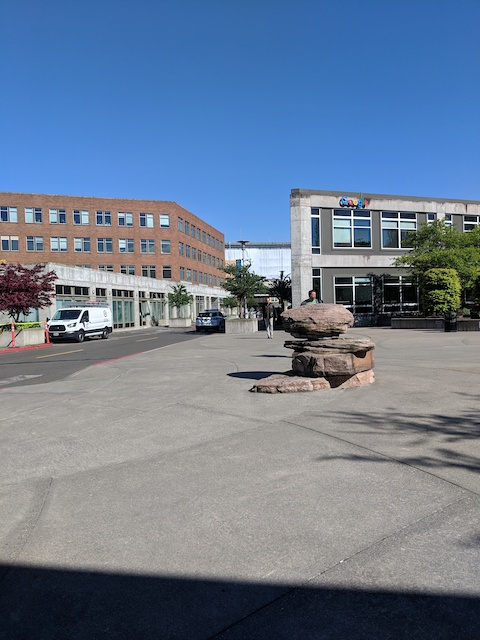
\includegraphics[width=0.32\textwidth]{google1.jpg}
  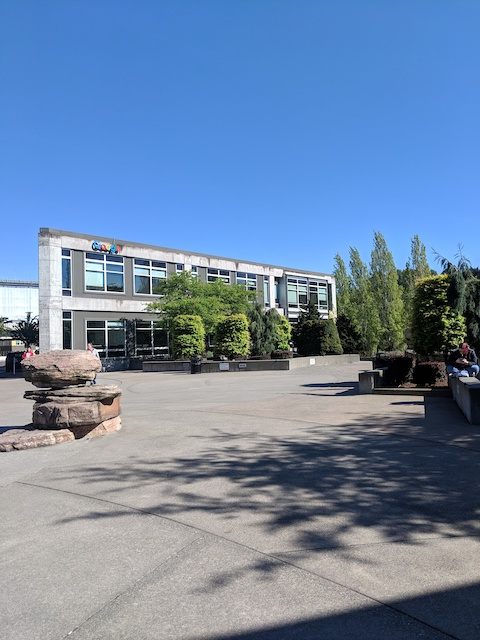
\includegraphics[width=0.32\textwidth]{google2.jpg}
  
  3 pictures of my office.
\end{center}

The center image was used as the reference coordinate system.

\begin{center}
  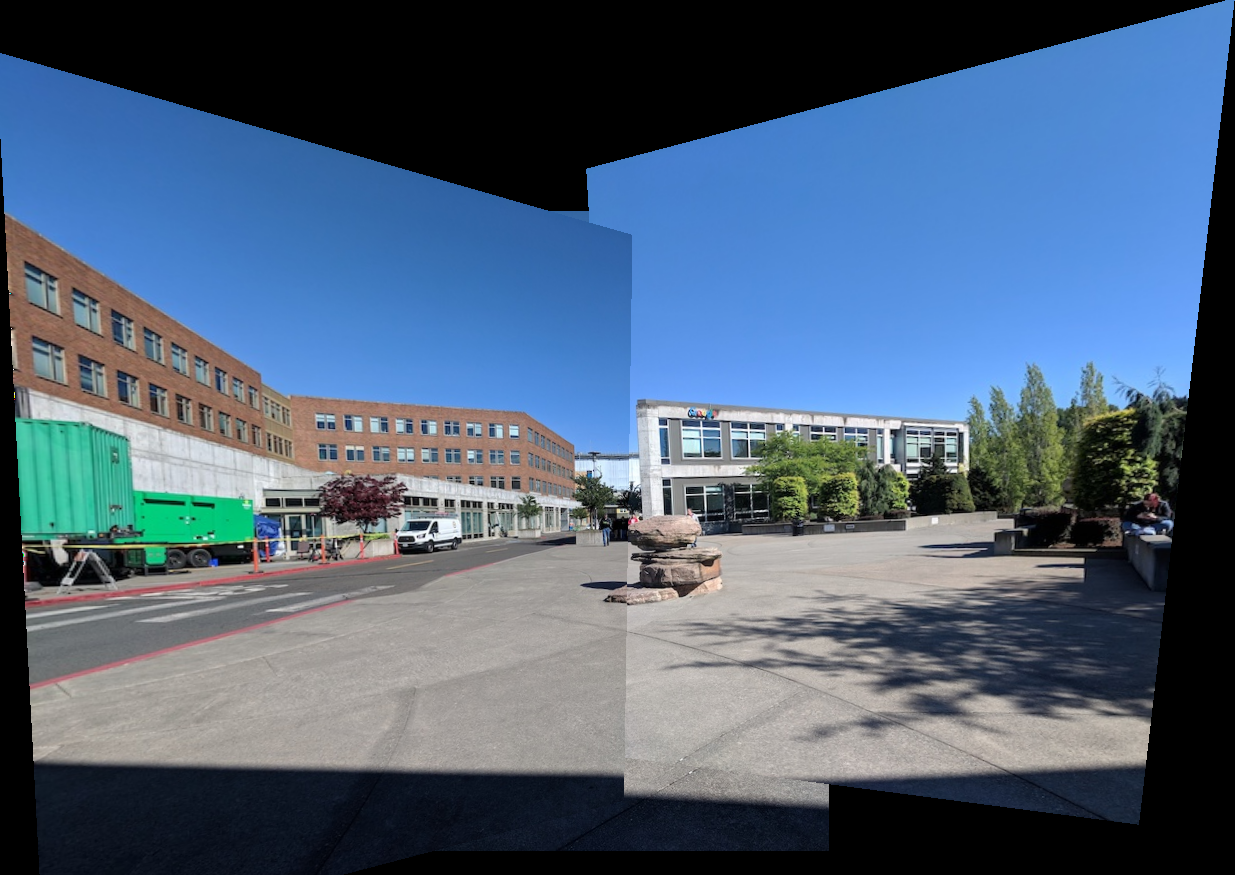
\includegraphics[width=\textwidth]{google_stitched.png} 
\end{center}

\section*{Whistle: Hanging}

To deal with the rotated image, I created a new 16-dimensional feature
descriptor. Consider a $9 \times 9$ window. Each dimension is the difference of
the green channel of a pixel on the border with that of center pixel. The
$0$-indexed dimensions correspond to the following pixels.

\begin{center}
  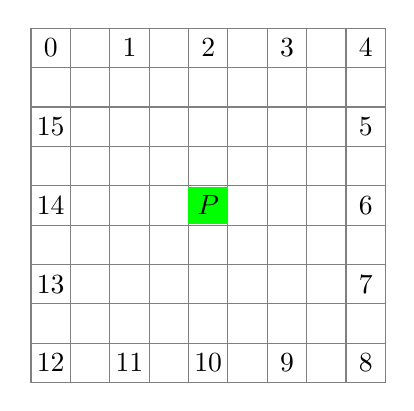
\begin{tikzpicture}
    \draw[step=0.5cm,color=gray] (-2.0,-2.0) grid (2.5,2.5);
    \node at (-1.75,2.25) {$0$};
    \node at (-0.75,2.25) {$1$};
    \node at (0.25,2.25) {$2$};
    \node at (1.25,2.25) {$3$};
    \node at (2.25,2.25) {$4$};
    \node at (2.25,1.25) {$5$};
    \node at (2.25,0.25) {$6$};
    \node at (2.25,-0.75) {$7$};
    \node at (2.25,-1.75) {$8$};
    \node at (1.25,-1.75) {$9$};
    \node at (0.25,-1.75) {$10$};
    \node at (-0.75,-1.75) {$11$};
    \node at (-1.75,-1.75) {$12$};
    \node at (-1.75,-0.75) {$13$};
    \node at (-1.75,0.25) {$14$};
    \node at (-1.75,1.25) {$15$};
    \node[fill=green] at (0.25,0.25) {$P$};
  \end{tikzpicture}
  \hspace{0.25cm}
\end{center}

Then, to make the distance metric rotation-invariant the distance between to
feature descriptors for pixels $P_1$ and $P_2$ is
\begin{equation}
  d\left(P_1,P_2\right) = \min_k\left(
    \sum_{j=0}^{15}\left\lvert
      P_1\left[j\right] - P_2\left[\left(j + 2k\right) \bmod 16\right]
      \right\rvert
    \right),
    \label{eqn:custom_metric}
\end{equation}
which computes the minimum $l_1$ distance over all $k\pi/4$ rotations.

\texttt{DESC\_SIZE} in \texttt{mainwindow.h} was changed to $16$.

\begin{center}
  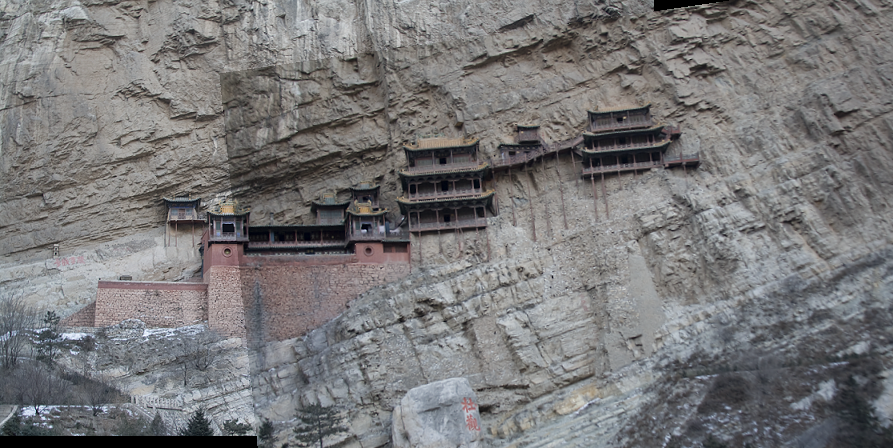
\includegraphics[width=\textwidth]{hanging.png}

  \texttt{Hanging1.png} and \texttt{Hanging2.png} by applying a 16-dimensional
  feature descriptor and Equation \ref{eqn:custom_metric}.
\end{center}

\section*{Whistle: Center-weighting}

In Section \ref{sec:stitch} the seam between the two stitched images is
apparent. Center-weighting can be used to make seam invisible.

\begin{center}
  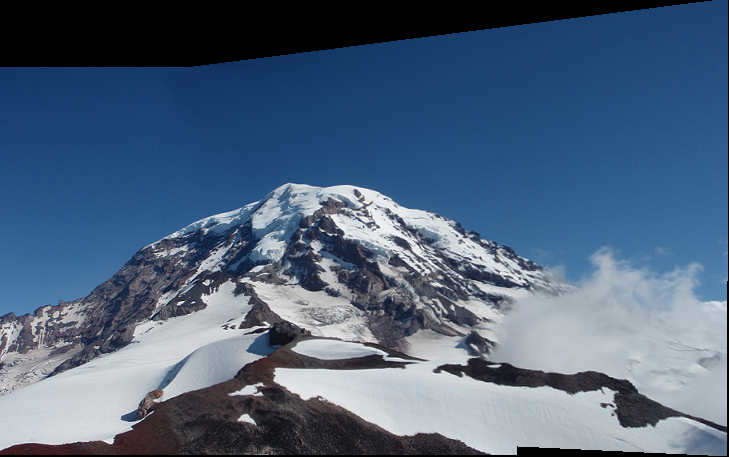
\includegraphics[width=\textwidth]{4_center_weighted.png}
  
  The result of stitching \texttt{Ranier1.png} and \texttt{Ranier2.png} with
  center-weighting.
\end{center}

The same can be done with the complete panorama.

\begin{center}
  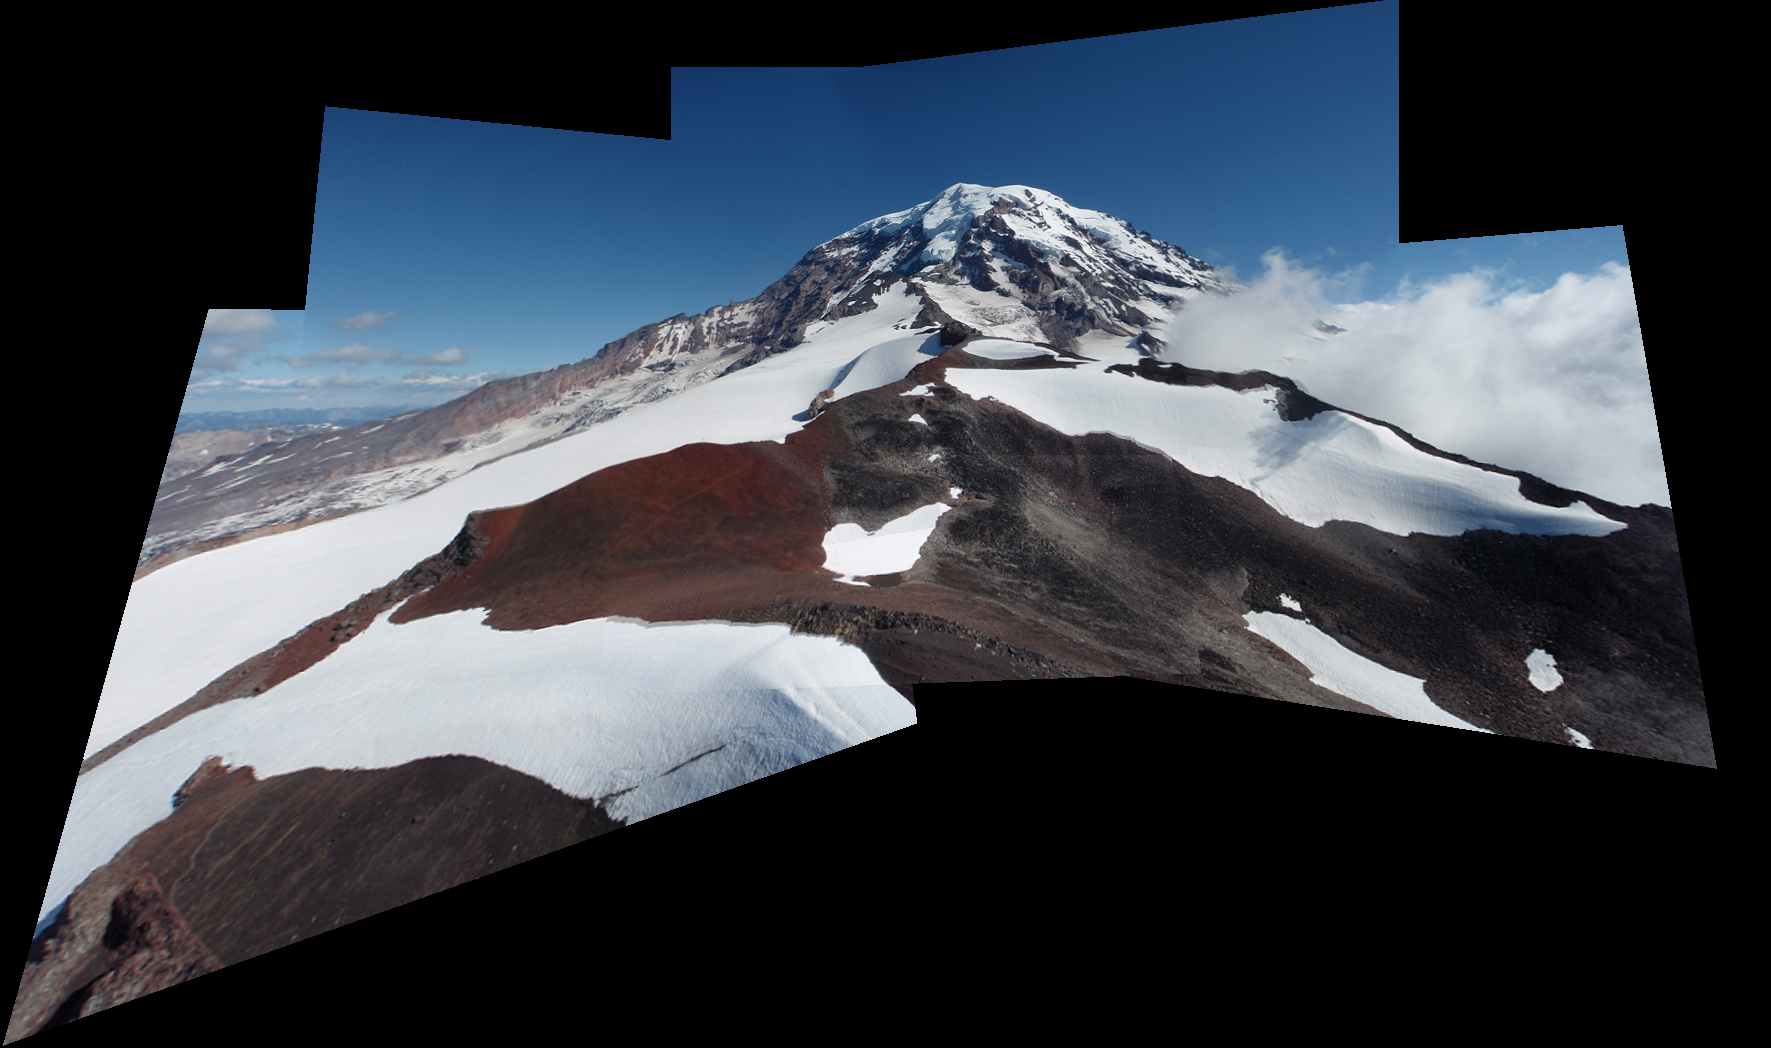
\includegraphics[width=\textwidth]{all_stitched_center_weighted.png}
  
  The result of stitching \texttt{Ranier1.png}, \texttt{Ranier2.png},
  \texttt{Ranier3.png}, \texttt{Ranier4.png}, \texttt{Ranier5.png}, and
  \texttt{Ranier6.png} with center-weighting.
\end{center}

\begin{center}
  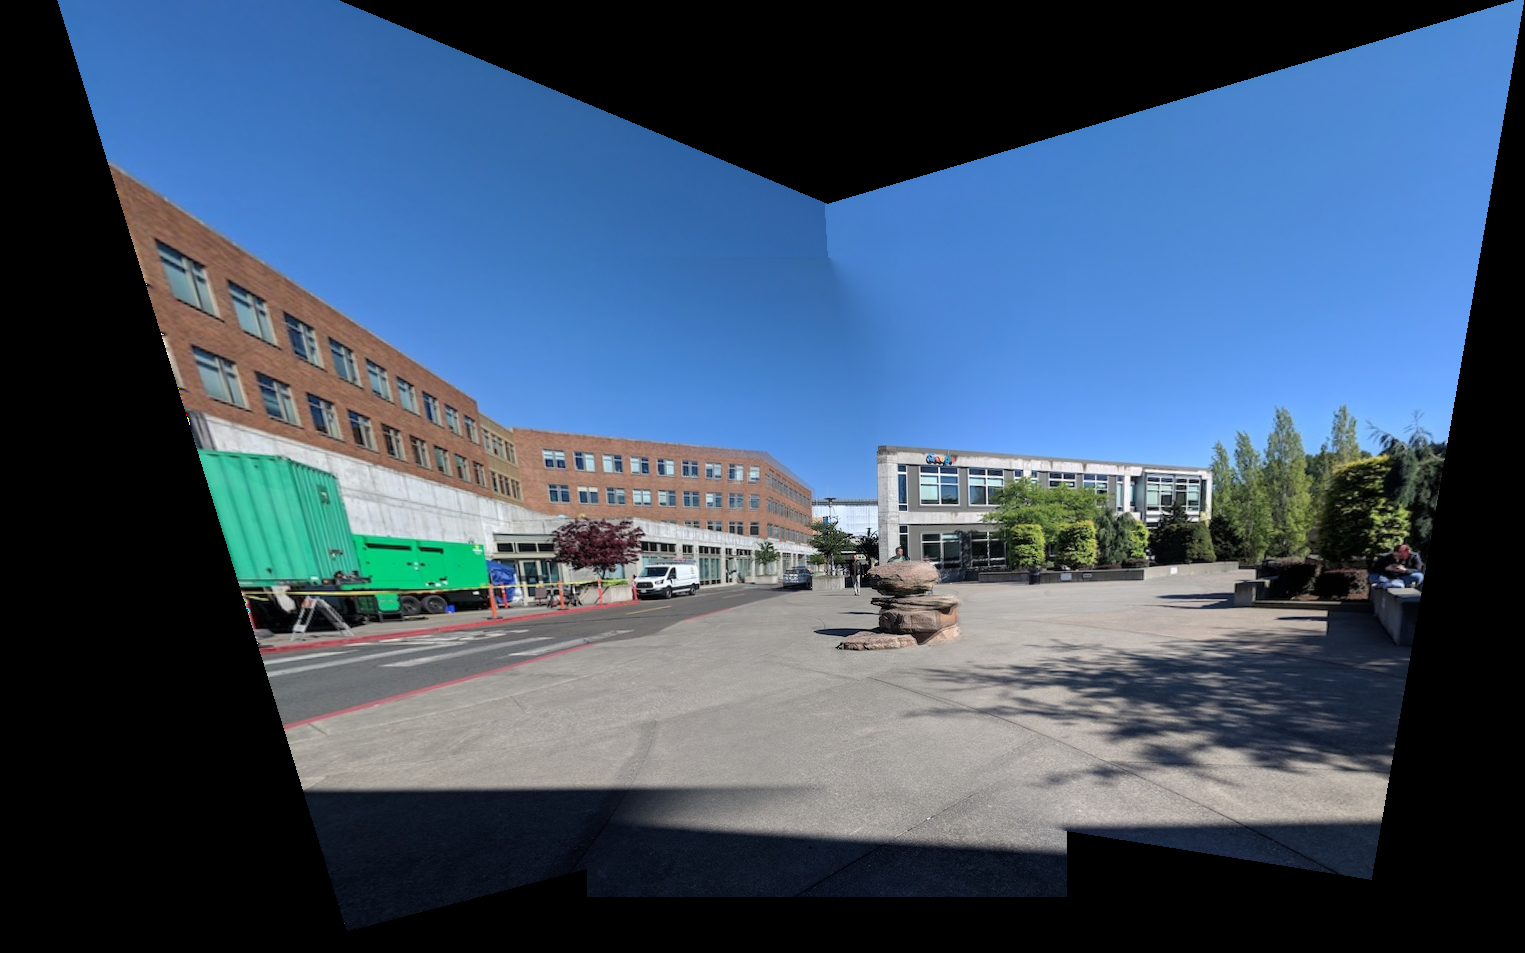
\includegraphics[width=\textwidth]{google_stitched_center_weighted.png}
  
  The Google campus with centering-weighting.
\end{center}

\begin{center}
  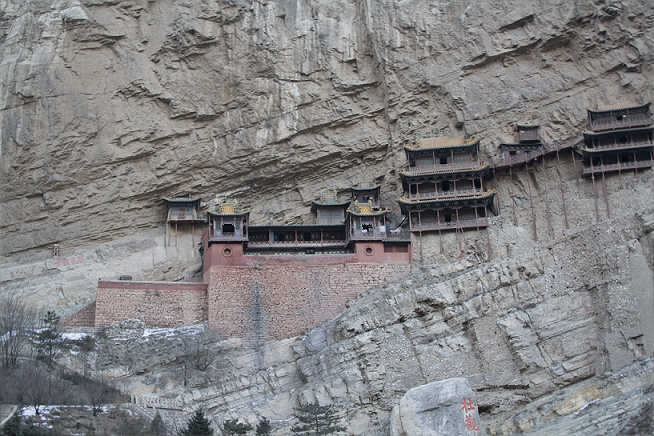
\includegraphics[width=\textwidth]{hanging_center_weighted.png}
  
  \texttt{Hanging1.png} and \texttt{Hanging2.png} stictched and center-weighted.
\end{center}

\section*{Appendix}

All code used to generate these images can be found at
\href{https://github.com/ppham27/cse576/blob/master/hw2}{\texttt{ppham27/cse576/hw2}}. The
embedded JPEG, PNG files, and the \LaTeX can be found in
\href{https://github.com/ppham27/cse576/blob/master/hw2/report}{\texttt{ppham27/cse576/hw2/report}}.

\end{document}
